\documentclass[twoside,11pt]{report}
\usepackage{tabularx} % extra features for tabular environment
\usepackage{amsmath} % improve math presentation
\usepackage{graphicx, subcaption} % takes care of graphic including machinery
% \usepackage{fancyhdr}
% \pagestyle{fancy}
% \setlength{\headheight}{14.0pt}
\usepackage[top=2.5cm, bottom=2.5cm, left=4.0cm, right=2.5cm]{geometry}
\usepackage{mathtools}
% \usepackage[margin=1in,letterpaper]{geometry} % decreases margins
\usepackage{xspace}
\usepackage{siunitx}
\usepackage{feynman}
\usepackage{pdflscape}
\usepackage{pifont}
\usepackage{booktabs}
\usepackage{ANA-FTAG-2020-08-PAPER-defs}
\usepackage{tikz-feynman} 
\usepackage[style=numeric-comp, sorting=none]{biblatex}
\addbibresource{ANA-FTAG-2020-08-PAPER.bib}
\addbibresource{Detector/Detector.bib}
\addbibresource{Reconstruction/Reconstruction.bib}
\addbibresource{DiHiggs/DiHiggs.bib}
\addbibresource{bib/ATLAS.bib}
\addbibresource{bib/CMS.bib}
\addbibresource{bib/DiHiggs_paper.bib}
\addbibresource{Theory/theory.bib}
\addbibresource{bib/ATLAS-useful.bib}
\addbibresource{bib/PubNotes.bib}
\addbibresource{bib/ConfNotes.bib}
\addbibresource{bib/ATLAS-SUSY.bib}
\addbibresource{bib/Int_note.bib}
\usepackage[final]{hyperref} % adds hyper links inside the generated pdf file


\PassOptionsToPackage{unicode}{hyperref}
\PassOptionsToPackage{naturalnames}{hyperref}
\usepackage[T1]{fontenc}
\usepackage{newtxtext,newtxmath}
\usepackage{setspace}
\usepackage{float}
\usepackage{makeidx}
\usepackage{titlesec}
\usepackage{multirow}
\usepackage{titling}
\newcommand\bjetineq{\mathop{\mbox{$b$ $\rm{jet}$}}}
\newcommand\bjetunder{\mathop{\footnotesize{\mbox{$b$ $\rm{jet}$}}}\normalsize}
\newcommand\cjetineq{\mathop{\mbox{$c$ $\rm{jet}$}}}
\newcommand\cjetunder{\mathop{\footnotesize{\mbox{$c$ $\rm{jet}$}}}\normalsize}
\setcounter{secnumdepth}{4}
\newcommand{\specialcell}[2][c]{%
 \begin{tabular}[#1]{@{}c@{}}#2\end{tabular}}
\newcommand{\changefont}{\fontsize{9}{11}\selectfont}
\newcommand{\changefontbig}{\fontsize{12}{14}\selectfont}
\titleclass{\subsubsubsection}{straight}[\subsection]

\newcounter{subsubsubsection}[subsubsection]
\renewcommand\thesubsubsubsection{\thesubsubsection.\arabic{subsubsubsection}}
\renewcommand\theparagraph{\thesubsubsubsection.\arabic{paragraph}} % optional; useful if paragraphs are to be numbered

\titleformat{\subsubsubsection}
  {\normalfont\normalsize\bfseries}{\thesubsubsubsection}{1em}{}
\titlespacing*{\subsubsubsection}
{0pt}{3.25ex plus 1ex minus .2ex}{1.5ex plus .2ex}

\makeatletter
\renewcommand\paragraph{\@startsection{paragraph}{5}{\z@}%
  {3.25ex \@plus1ex \@minus.2ex}%
  {-1em}%
  {\normalfont\normalsize\bfseries}}
\renewcommand\subparagraph{\@startsection{subparagraph}{6}{\parindent}%
  {3.25ex \@plus1ex \@minus .2ex}%
  {-1em}%
  {\normalfont\normalsize\bfseries}}
\def\toclevel@subsubsubsection{4}
\def\toclevel@paragraph{5}
\def\toclevel@paragraph{6}
\def\l@subsubsubsection{\@dottedtocline{4}{7em}{4em}}
\def\l@paragraph{\@dottedtocline{5}{10em}{5em}}
\def\l@subparagraph{\@dottedtocline{6}{14em}{6em}}
\makeatother
\newcommand*{\App}[1]{Appendix~#1\xspace}
\newcommand*{\Eqn}[1]{Eq.~#1\xspace}
\newcommand*{\Fig}[1]{Figure~#1\xspace}
\newcommand*{\Refn}[1]{Ref.~#1\xspace}
\newcommand*{\Sect}[1]{Section~#1\xspace}
\renewcommand*{\Tab}[1]{Table~#1\xspace}
\newcommand*{\Apps}[2]{Appendices~#1 and #2\xspace}
\newcommand*{\Eqns}[2]{Eqs.~#1 and #2\xspace}
\newcommand*{\Figs}[2]{Figures~#1 and #2\xspace}
\newcommand*{\Refns}[2]{Refs.~#1 and #2\xspace}
\newcommand*{\Sects}[2]{Sections~#1 and #2\xspace}
\newcommand*{\Tabs}[2]{Tables~#1 and #2\xspace}
\newcommand*{\Apprange}[2]{Appendices~#1--#2\xspace}
\newcommand*{\Eqnrange}[2]{Eqs.~#1--#2\xspace}
\newcommand*{\Figrange}[2]{Figures~#1--#2\xspace}
\newcommand*{\Refrange}[2]{Refs.~#1--#2\xspace}
\newcommand*{\Sectrange}[2]{Sections~#1--#2\xspace}
\newcommand*{\Tabrange}[2]{Tables~#1--#2\xspace}
\newcommand*{\hhtobbyy}{\ensuremath{\HH\rightarrow\bbyy}\xspace}
\newcommand*{\hhtobbtt}{\ensuremath{\HH\rightarrow\bbtautau}\xspace}
\newcommand*{\lambdaHHH}{\ensuremath{\lambda_{HHH}}\xspace}
\newcommand*{\lambdaSM}{\ensuremath{\lambda_{\mathrm{SM}}}\xspace}
\newcommand*{\kappalambda}{\ensuremath{\kappa_\lambda}\xspace}
\newcommand*{\cgghh}{\ensuremath{c_{gghh}}\xspace}
\newcommand*{\ctthh}{\ensuremath{c_{tthh}}\xspace}

\setcounter{secnumdepth}{4}
\setcounter{tocdepth}{4}

\restylefloat*{figure}
\hypersetup{
	colorlinks=true, % false: boxed links; true: colored links
	linkcolor=blue, % color of internal links
	citecolor=blue, % color of links to bibliography
	filecolor=magenta, % color of file links
	urlcolor=blue 
}


\begin{document}

\Large{3.1\ Title of Representative Academic Achievements}\\
\newline
\normalsize
Search for resonant and non-resonant Higgs boson pair
production in the \bbtautau\ decay channel using 13 TeV $pp$ collision data from the ATLAS detector\\
\newline
\Large{3.2\ Abstract of Representative Academic Achievement}\\
\normalsize
    \newline
    I have worked on a search for Higgs boson pair production in events with 
    two $b$-jets and two $\tau$-leptons is presented, using a proton--proton collision 
    data set with an integrated luminosity of $139~\text{fb}^{-1}$ collected 
    at $\sqrt{s}=13~\text{TeV}$ by the ATLAS experiment at the LHC. Higgs boson pairs 
    produced non-resonantly or in the decay of a narrow-width scalar resonance in 
    the mass range 251 to 1600~GeV are targeted. Events in which at least one $\tau$-lepton 
    decays hadronically are considered, and multivariate discriminants are used to extract the signals. 
    No significant excess of events above the expected background is observed in the non-resonant search. 
    Observed (expected) upper limits are set at the 95\% confidence-level on the 
    non-resonant Higgs boson pair production cross-section of 4.7 (3.9) times 
    the Standard Model prediction, which sets the \textbf{current world-best 
    observed limit}. 
    Upper limits are also set on the resonant signal of Higgs boson pair production 
    cross-section between 23 and 920~fb (12 and 840~fb), depending on the heavy resonance mass.
    The largest excess in the resonant search is observed at a resonance mass of 
    1~\TeV, with a local (global) significance of $3.0~\sigma$ ($2.0^{+0.4}_{-0.2}~\sigma$). 
    The excess of $2~\sigma$ is already statistically significant, 
    and could possibly provide \textbf{hint for new physics}, and may guide future search for beyond 
    Standard Model physics (BSM) 
    for years to come, as the more data one has, the stronger one can prove or disprove the anomaly.\\
    \newline
\Large{3.3\ Main Content of the Representative Academic Achievements}\\
\normalsize
    \newline
    The discovery of a Higgs boson ($H$) of mass around 125~GeV 
    has inspired a vast number of measurements and searches by the ATLAS 
    and CMS collaborations at the Large Hadron Collider (LHC).
    To date, all measurements of Higgs boson properties are consistent to
    the Standard Model (SM) predictions,
    and no unexpected particles or Higgs boson decay modes have been observed.
    One of the most important properties of Higgs boson is that Higgs boson
    interacts with itself, as determined by the Higgs potential,
    makes the Higgs boson pair production (di-Higgs production) possible.
    In the non-resonant production of di-Higgs, 
    the gluon--gluon fusion (ggF) process contributes approximately 90\% of 
    the total cross-section. The leading-order (LO) contributions to the ggF $HH$ production are 
    the `triangle diagram', which occurs via the Higgs boson self-coupling, 
    and the heavy quark `box diagram', which occurs via two 
    fermion--fermion--Higgs vertices.
    These two diagrams are shown in Figure~\ref{fig:SM_diagrams_o4}.
    %\usepackage[utf8]{inputenc}
%\usepackage{tikz}
%\usepackage[compat=1.1.0]{tikz-feynman}
%\usepackage{subcaption}
%\usepackage{geometry}

\definecolor{hh_pink}{HTML}{F2385A}
\definecolor{hh_blue}{HTML}{343844}
\definecolor{hh_med_turq}{HTML}{36B1BF}
\definecolor{hh_lgt_turq}{HTML}{4AD9D9}
\definecolor{hh_whte}{HTML}{E9F1DF}
\definecolor{hh_yllw}{HTML}{FDC536}
%\definecolor{hh_gren}{HTML}{125125}
\definecolor{hh_gren}{HTML}{00CC00}


%\usepackage[EULERGREEK]{sansmath}
%\usepackage{floatrow}
%\DeclareFloatFont{henry}{\sffamily\sansmath}
%\floatsetup[figure]{font=henry}

\begin{figure}[tbh!]
    \centering                      
    \begin{subfigure}[t]{0.5\textwidth}
        \centering
        \begin{tikzpicture}
            \begin{feynman}
                \vertex(g1) at (-3.3, -1.25) {\(\mathbf{g}\)};
                \vertex(g2) at (-3.3, 1.25) {\(\mathbf{g}\)};
                
                \vertex (t1) at (-1.25, -1.25);
                \vertex (t2) at (-1.25, 1.25);
                \vertex (t3) at (0.92, 0);
                
                \vertex (h1) at (2.5, 0);
                \vertex (h2) at (3.7, 1.25) {\(\mathbf{H}\)};
                \vertex (h3) at (3.7, -1.25) {\(\textbf{H}\)};

                \diagram*{
                    (g1) -- [gluon, thick] (t1),
                    (g2) -- [gluon, thick] (t2),
                    
                    (t1) -- [fermion, thick] (t2) -- [fermion, thick] (t3) -- [fermion, thick] (t1),
                    
                    (t3) -- [scalar, thick, edge label'=\(\textbf{H}\)] (h1) -- [scalar, thick] {(h2), (h3)}
                    
                };
                
            \end{feynman}

        \filldraw [hh_med_turq] (1.0, 0) circle (3pt);
        \node[hh_med_turq, scale=1.25] at (1.0, 0.6) {\(c_{tth}\)};
        \filldraw [hh_pink] (2.5, 0) circle (3pt);
        \node[hh_pink, scale=1.25] at (2.5, 0.6) {\(c_{hhh}\)};
        
        \end{tikzpicture}
        %\caption{Triangle diagram with $t\bar{t}H$ and $HHH$ couplings}
        \label{fig:SM_diagrams_o4:triangle}
        \end{subfigure}%
        \begin{subfigure}[t]{0.50\textwidth}
        \centering
        \begin{tikzpicture}
            \begin{feynman}
                
                \vertex(g1) at (-3.3, -1.25) {\(\mathbf{g}\)};
                \vertex(g2) at (-3.3, 1.25) {\(\mathbf{g}\)};
                
                \vertex (t1) at (-1.25, -1.25);
                \vertex (t2) at (-1.25, 1.25);
                \vertex (t3) at (1.25, 1.25);
                \vertex (t4) at (1.25, -1.25);
            
                \vertex (h1) at (3.3, -1.25) {\(\mathbf{H}\)};
                \vertex (h2) at (3.3, 1.25) {\(\mathbf{H}\)};

                \diagram*{
                    (g1) -- [gluon, thick] (t1),
                    (g2) -- [gluon, thick] (t2),
                    (t1) -- [fermion, thick] (t2) -- [fermion, thick] (t3) -- [fermion, thick] (t4) -- [fermion, thick] (t1),
                    (t3) -- [scalar, thick] (h2),
                    (t4) -- [scalar, thick] (h1)
                    
                };
                
            \end{feynman}

        \filldraw [hh_med_turq] (1.25, 1.25) circle (3pt);
        \node[hh_med_turq, scale=1.25] at (1.65, 1.65) {\(c_{tth}\)};
        \filldraw [hh_med_turq] (1.25, -1.25) circle (3pt);
        \node[hh_med_turq, scale=1.25] at (1.65, -0.85) {\(c_{tth}\)};

        \end{tikzpicture}
    %\caption{Box diagram with $t\bar{t}H$ coupling}
    \label{fig:SM_diagrams_o4:box}
    \end{subfigure} \\

    \caption[Feynman diagrams, gluon-gluon fusion di-Higgs production]{SM leading-order Feynman diagrams for Higgs boson pair production through gluon-gluon fusion.}% In SM, $c_{tth}=c_{hhh}=1$ and $c_{tthh}=c_{ghh}=c_{gghh}=0$.}
    \label{fig:SM_diagrams_o4}
\end{figure}

    These diagrams interfere destructively, leading to a small SM ggF $HH$ cross-section, 
    which is predicted to be 31.1~fb at next-to-next-to-leading (NNLO) order 
    in $\alpha_s$ and including an approximation of finite top-quark-mass effects, 
    for $m_H=125$~GeV and 
    $\sqrt{s}=13$~\TeV. 
    The vector boson fusion (VBF) process provides a sub-leading source 
    of $HH$ production in the SM, and has a cross-section of 1.73~fb. 
    Due to this small cross-section 
    and provided the current LHC data set, 
    the observation of SM non-resonant $HH$ production is an extremely difficult
    and ambitious task, and has become one of the \textbf{main goals of LHC analysis},
    and one of the steer and motivation for the future upgrade of the LHC. 

    Nevertheless the small cross-section, the $HH$ production cross-section can be enhanced by many BSM theories.
    Due to the destructive interference between the triangle diagram and the box diagram,
    non-resonant $HH$ production provides a \textbf{sensitive probe} of the Higgs boson trilinear 
    self-coupling and the shape of the Higgs field potential, 
    which have \textbf{crucial implications} for the stability of the electroweak vacuum, 
    baryogenesis, and inflation. 
    Modifications to the non-resonant $HH$ cross-section occur in BSM scenarios with new, 
    light, coloured scalars, composite Higgs models, 
    theoretical scenarios with couplings between pairs of top-quarks and pairs of Higgs bosons, 
    as well as models with a modified coupling of the Higgs boson to the top-quark. 
% Previous searches for non-resonant $HH$ production by ATLAS and CMS have been performed in 
% the $b\bar b\tau^+\tau^-$, $b\bar b\gamma\gamma$, $b\bar bb\bar b$, $b\bar b\ell^+\nu\ell^-\nu$ decay channels, 
% by ATLAS in the $b\bar bqq\ell\nu$, $WW^*\gamma\gamma$ 
% and $WW^*WW^*$ decay channels, and by CMS in the $b\bar bWW^*/b\bar bZZ^*$ 
% decay channel. In the $b\bar b\tau^+\tau^-$ decay channel, ATLAS and CMS set observed (expected) upper 
% limits on the non-resonant $HH$ production cross-section of 12.7 (14.8) 
% and 30 (25) times the SM expectation using 36.1~\ifb\ and 35.9~\ifb\ of 
% 13~TeV $pp$ collision data, respectively. Using these data sets, ATLAS and CMS performed combinations of 
% several search channels improving these observed (expected) limits to 6.9 (10) 
% and 22.2 (12.8) times the SM expectation, respectively. 
% ATLAS and CMS recently published searches for $HH$ production in the $b\bar b\gamma\gamma$ 
% decay mode using their full Run-2 $pp$ collision data sets, which set observed (expected) 
% upper limits on the SM non-resonant $HH$ cross-section of 4.1 (5.5) and 5.2 (7.7) times the SM expectation, 
% respectively. CMS also recently published a search for $HH$ production 
% in the $b\bar bb\bar b$ decay mode using their full Run-2 $pp$ collision data set, 
% which set an observed (expected) upper limit on the SM non-resonant $HH$ cross-section of 3.6 (7.3) times 
% the SM expectation.% in the $b\bar b\tau^+\tau^-$, $b\bar b\gamma\gamma$, $b\bar bb\bar b$, $b\bar bVV^*$, $WW^*\gamma\gamma$, and $VV^*VV^*$ decay channels.
    Various BSM scenarios predict heavy resonances that can decay to pairs of Higgs bosons. 
    These BSM resonances include heavy Higgs bosons from extended Higgs sectors such as two Higgs doublet 
    models (2HDMs), the minimal supersymmetric extension of the 
    SM and composite Higgs models. Heavy resonances that decay 
    to pairs of Higgs bosons also include spin-0 radions and spin-2 gravitons from the 
    Randall--Sundrum model, and stoponium states in supersymmetric models. 
    % Searches for resonant $HH$ production have been performed in many final states by ATLAS and CMS, 
    % and no significant excesses have been 
    % observed.% EXOT-2016-31

    The search for non-resonant and resonant $HH$ production is conducted
    in the final state with two jets containing $b$-hadrons ($b$-jets) and two $\tau$-leptons,
    as referred to the $bb\tau\tau$ channel. 
    The $bb\tau\tau$ channel has a sizeable branching ratio of 7.3\% as predicted by the SM, 
    and has relatively low backgrounds.
    These advantages make the $bb\tau\tau$ one of the \textbf{most sensitive $HH$ search channels}. 
    In the search for non-resonant $HH$ production, the signal is assumed to have SM-like kinematics, 
    and the search is optimised for maximum sensitivity to the 
    cross-section rather than the Higgs boson self-coupling. 
    A narrow-width CP-even scalar particle with a mass between 251 and 
    1600~GeV is used as the benchmark model for the resonant signal. 
    Decay modes in which both $\tau$-leptons decay hadronically, 
    and in which one decays hadronically and the other leptonically, 
    are both considered.
    The presence of a hadronically-decaying $\tau$ is determined by its
    visible decay products. 
    Events are categorised based on the type of trigger that accepted the event, 
    and are required to contain two oppositely charged hadronically-decaying $\tau$ 
    and two $b$-tagged jets in the hadhad final state, 
    or an electron or muon and an oppositely charged hadronically-decaying $\tau$ and 
    two $b$-tagged jets in the lephad final state. 
    % Signal events also contain neutrinos from the decay of $\tau$-leptons and $b$-hadrons, 
    % which manifest themselves as missing momentum transverse to the beamline. 
    Backgrounds in this search include top-quark pairs, single top-quarks, 
    $W$ and $Z$~bosons in association with jets, diboson processes, 
    single Higgs bosons, and multi-jet production. 
    In some background events, quark- or gluon-initiated jets are 
    misidentified as the $\tau$-lepton. 
    The selected events are tested for the presence of the signal 
    by performing profile-likelihood fits to multivariate discriminant distributions. 
    The search is performed using the full Run~2 $pp$ collision data set,
    delivered between 2015 and 2018 at a centre-of-mass energy $\sqrt{s}=13$~TeV by the LHC. 
    The data were collected by the ATLAS detector 
    and correspond to an integrated luminosity of 139~\ifb. 
    No significant excess of signal has been observed in the non-resonant $HH$ production,
    therefore upper limits are set on the cross section. 
    Observed (expected) upper limits are set at the 95\% confidence-level on the 
    non-resonant Higgs boson pair production cross-section of 4.7 (3.9) times 
    the Standard Model prediction, as shown in Table~\ref{sec:fit:tab:SMCombinedLimits}.
    \begin{table}[htbp]
    \centering
    \begin{tabular}{|c|c|c|c|c|c|c|}
    \hline
    & Observed & $-2\sigma$ & $-1\sigma$ & Median & $+1\sigma$ & $+2\sigma$\\
    % \hline
    % $\sigma_{ggF}$ [fb] & 130.41   &    59.05   &    79.27   &    110.02    &    153.11  &    205.25 \\
    % \hline
    % $\sigma_{ggF}$ StatOnly [fb] & 83.68   &    46.60  &     62.56  &     86.82   &    120.83  &    161.98 \\ 
    % \hline
    % $\mu_{ggF}=\sigma_{ggF}/\sigma_{ggF}^\text{SM}$ & 4.75   & 2.11   &    2.84  &     3.95  &    5.49  &    7.36 \\ 
    % \hline
    % $\mu_{ggF}=\sigma_{ggF}/\sigma_{ggF}^\text{SM}$ StatOnly & 2.69   & 1.50   &    2.01   &    2.80   &    3.89  &    5.22 \\ 
    % \hline
    \hline
    $\sigma_\text{ggF+VBF}$ [fb] & 135.27   & 61.35  &   82.36  &   114.31   &   159.08  &   213.26 \\ 
    \hline
    $\sigma_\text{ggF+VBF}$ StatOnly [fb] & 85.58  &    48.45  &   65.04  &  90.27  &   125.63  &   168.41 \\ 
    \hline
    $\mu_\text{ggF+VBF}$ & 4.65  &     2.08   &    2.79   &    3.87  &    5.39  &    7.22 \\ 
    \hline
    $\mu_\text{ggF+VBF}$ StatOnly & 2.61   &    1.48   &    1.98   &    2.75   &    3.83  &    5.14 \\ 
    \hline
    \end{tabular}
    \caption{95\% C.L. expected and observed limit on the non-resonant HH production cross-section 
    assuming SM kinematics using \lephad and \hadhad combined fit.
    The signal strength is with respect to the 
    SM cross-section, i.e.\ 
    $\mu_\text{ggF+VBF}=\sigma_\text{ggF+VBF}/\sigma_\text{ggF+VBF}^\text{SM}$.
    The `StatOnly' indicates the limits are calculated with only statistical uncertainty,
    and if not specified, the limits are obtained with full systematics.}
    \label{sec:fit:tab:SMCombinedLimits}
    \end{table}

    Upper limits are also set on the resonant signal of Higgs boson pair production 
    cross-section between 23 and 920~fb (12 and 840~fb),
    as shown in Figure~\ref{fig:CombinedLimits}.
    \newline

    \begin{figure}[htbp]
        \centering
        \includegraphics[width=.8\textwidth]{figures/results/HH/Combined/CombSysts_21072021.pdf}
        \caption{95\% C.L. expected and observed limits on the resonant HH production cross-section as a function of the resonance mass. 
        The dashed lines show the expected limits, while the solid lines show the observed limits. 
        Black, red and blue represents the upper limit from combination, \lephad channel and \hadhad channel, respectively.}
        \label{fig:CombinedLimits}
        \end{figure}
    % This exciting results profit from improved hadronically-decaying $\tau$ 
    % and $b$-jet reconstruction and identification, more sophisticated multivariate techniques 
    % used to target the resonant signal hypotheses, and new background estimation techniques.






\Large{3.4\ Title of Representative Academic Achievements}\\
\newline
\normalsize
Measurement of the $c$-jet mistagging efficiency in $t\bar{t}$~events 
using $pp$ collision data at $\sqrt{s}=13$~$\text{Te\kern -0.1em V}$ collected with the ATLAS detector\\
\newline
\Large{3.5\ Abstract of Representative Academic Achievement}\\
\normalsize
\newline
    I have investigated a technique to measure the  efficiency 
    with which $c$-jets are mistagged as $b$-jets (mistagging efficiency) 
    using $t\bar{t}$ events, where one of the $W$
    bosons decays into an electron or muon and a neutrino and the other
    decays into a quark-antiquark pair. The measurement utilises the relatively large
    and known $W\to cs$ branching ratio, which allows a measurement to be made
    in an inclusive $c$-jet sample.  The data sample used was
    collected by the ATLAS detector at $\sqrt{s} = 13$~$\text{Te\kern -0.1em V}$ 
    and corresponds to an integrated luminosity of 139~fb$^{-1}$.  
    Events are reconstructed using a kinematic likelihood technique
    which selects the mapping between jets and $t\bar{t}$
    decay products that yields the highest likelihood value.
    The distribution of the $b$-tagging discriminant for jets from the hadronic $W$ 
    decays in data is compared with that in simulation to extract the mistagging efficiency 
    as a function of jet transverse momentum. 
    The total uncertainties are in the range 3\%--17\%. 
    The measurements generally agree with 
    those in simulation but there are some differences 
    in the region corresponding to the most stringent $b$-jet tagging requirement.
    The calibration results on the \btagging\ algorithm have become the 
    \textbf{official recommendation for
    all ATLAS users} who apply \btagging\ in their analyses. 
    \newline
\Large{3.6\ Main Content of the Representative Academic Achievements}\\
\normalsize
\newline
    The algorithms for the identification of jets containing $b$-hadrons,
    also known as \btagging\ algorithms,  
    constitute an important tool for the analysis of the data collected by the ATLAS 
    experiment at the Large Hadron Collider (LHC).
    Such algorithms play a \textbf{crucial role} in a large number of Standard Model (SM) 
    precision measurements, Higgs boson measurements, and searches for supersymmetry
    and other exotic phenomena. 
    Jets that contain a $b$-hadron are distinguished from other jets that
    contain a $c$-hadron or only light-flavour hadrons mainly by the
    larger mass and longer lifetime of the $b$-hadron.  The \btagging\ 
    algorithm studied is called DL1r, and is an updated
    version of the DL1 tagger, which combines the output of the 
    low-level taggers into a single discriminant by using a deep neural network.
    DL1r adds the result of the RNNIP algorithm, which is
    based on a recurrent neural network exploiting the correlation between
    the tracks' impact parameters. 

    The performance of the
    \btagging\ algorithms depends crucially on whether the jets that are
    identified contain $b$-hadrons (\bjets), $c$-hadrons (\cjets), or neither
    of them (light-flavour jets).
    The Monte Carlo (MC) simulation provides an estimate of the probabity that
    a jet fulfils the requirements of the \btagging\ algorithm i.e.\ the
    tagging efficiency  for \bjets\ and the mistagging
    efficiency for \cjets\ and light-flavour jets. However, since the
    simulation is not perfect, the (mis)tagging efficiency must be
    measured in data. Simulation to data scale factors (SFs), which are defined as the ratio of
    the efficiency measured in data to that in simulation, are used as a
    correction to the simulation, assuming that the SFs
    are independent of the physics process. Analyses that use
    \btagging\  apply a weight to each simulated event, derived as the
    product of the SFs for all jets for which a tagging
    requirement is made.

    % Measurements of the SFs have been made using \ttbar\
    % events for \bjets and inclusive jet 
    % events for light-flavour jets. Measurements of
    % SFs for \cjets\ using proton--proton (\(pp\))
    % collision data at $\sqrt{s}= 7$~\TeV, described in Ref.,
    % use two methods to measure the mistagging efficiency of \cjets. One
    % technique uses the production of a $W$ boson in association with a  \cjet\
    % that decays semi-muonically and the other identifies a $D^*$ meson within \cjets\ by explicitly
    % reconstructing the meson decay chain $D^{*+} \to D^{0} \pi^+ \to
    % K^{-}\pi^+\pi^+$.

    A technique is used to measure the inclusive \cjet\ mistagging efficiency by means of a
    \cjet\ sample that is derived from \ttbar\ events.  The measurement uses a
    \(pp\) collision dataset which was collected with the ATLAS
    detector during 2015--2018 and corresponds to an integrated luminosity of 
    \lumi.  A likelihood-based method is used to select a high-purity \ttbar\
    sample in which one of the $W$ bosons originating from the
    top-quark decay $t\to W b$ decays leptonically 
    into an electron or a muon plus the
    corresponding neutrino and the other decays hadronically. The 
    branching ratio of a $W$ boson to 
    final states containing a charm-quark, which is approximately 
    33\%, allows the \cjet\ mistagging efficiency of the data to be
    determined as a function of jet transverse momentum by fitting
    simulated event samples to the data sample.
    The technique has the advantage that it does not depend on a specific
    hadron decay chain topology.

    The scale factors are shown in Figure~\ref{fig:Dec_SF_PFlow_DL1r} for the PFlow jets
    with the DL1r tagger. 
    The tighter working points (60\%, 70\%) show larger uncertainties and bigger deviation from 1, while
    the looser working points (77\%, 85\%) have much smaller uncertainty and the simulation is able to 
    recover the data well due to more abundant events statistics.
    In most of the working points the systematic uncertainties dominate 
    in the low-\pt\ bins (\pt\ < 150) and the statistical error, represented by the error bars on the 
    markers, become more important in the last bin. 
    \newline
    \begin{figure}[htbp]
    \centering
    \begin{subfigure}[t]{.35\linewidth}
    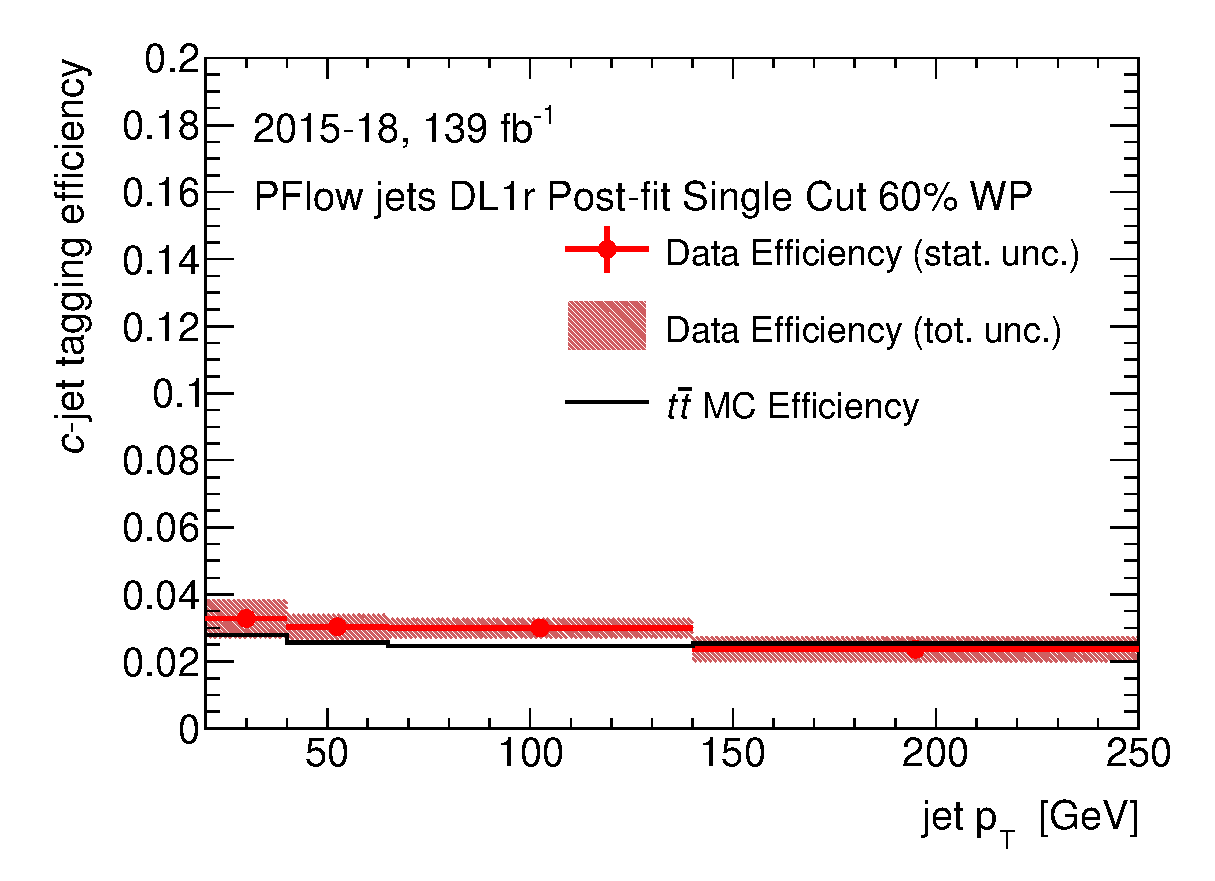
\includegraphics[width=1\textwidth]{FTAG_plots/DL1rallPFlowDec/eff60.eps}
    \caption{60\% working point}
    \end{subfigure}
    \begin{subfigure}[t]{.35\linewidth}
    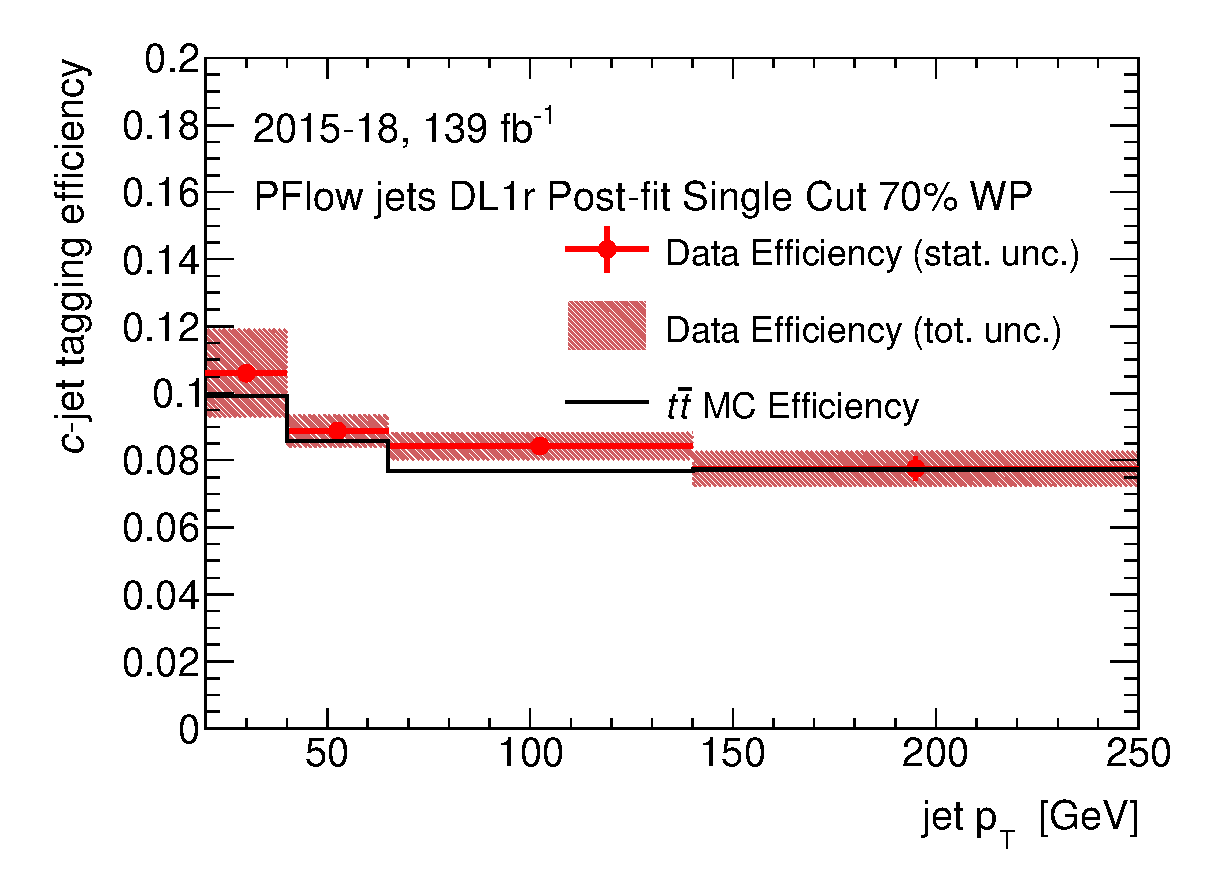
\includegraphics[width=1\textwidth]{FTAG_plots/DL1rallPFlowDec/eff70.eps}
    \caption{70\% working point}
    \end{subfigure}
    \begin{subfigure}[t]{.35\linewidth}
    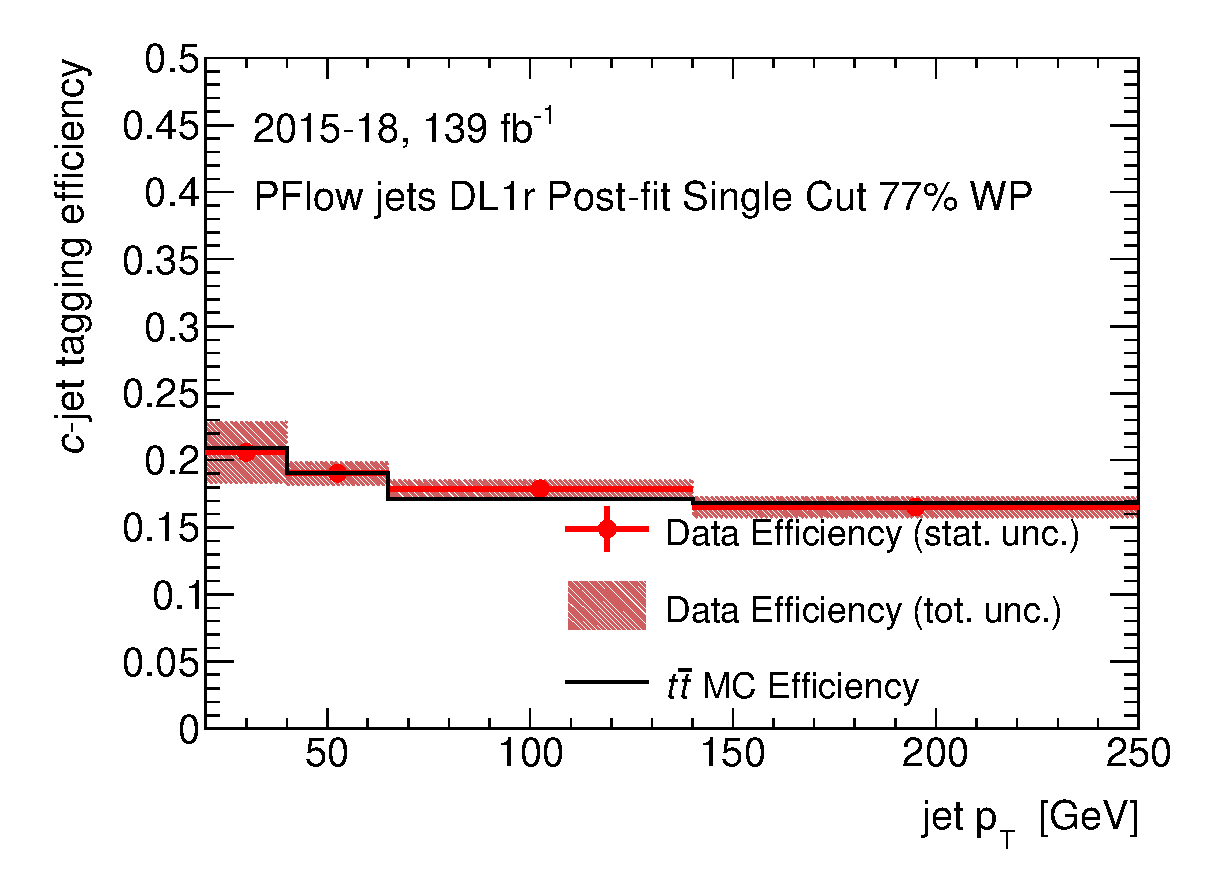
\includegraphics[width=1\textwidth]{FTAG_plots/DL1rallPFlowDec/eff77.eps}
    \caption{77\% working point}
    \end{subfigure}
    \begin{subfigure}[t]{.35\linewidth}
    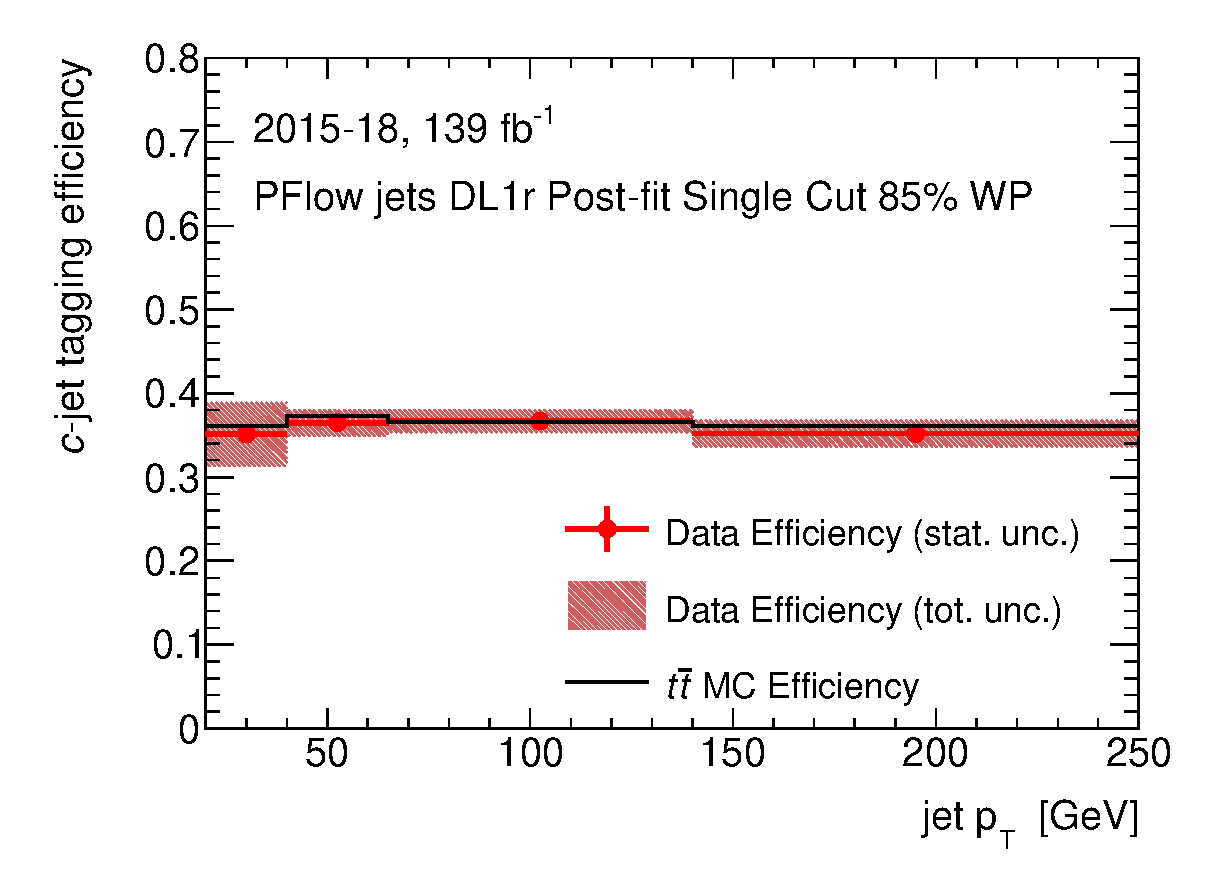
\includegraphics[width=1\textwidth]{FTAG_plots/DL1rallPFlowDec/eff85.eps}
    \caption{85\% working point}
    \end{subfigure}
    \caption{Charm-jet efficiencies for the PFlow jets collection with
    the DL1r tagger.} \label{fig:Dec_eff_PFlow_DL1r}
    \end{figure}

    \begin{figure}[htbp]
    \centering
    \begin{subfigure}[t]{.35\linewidth}
    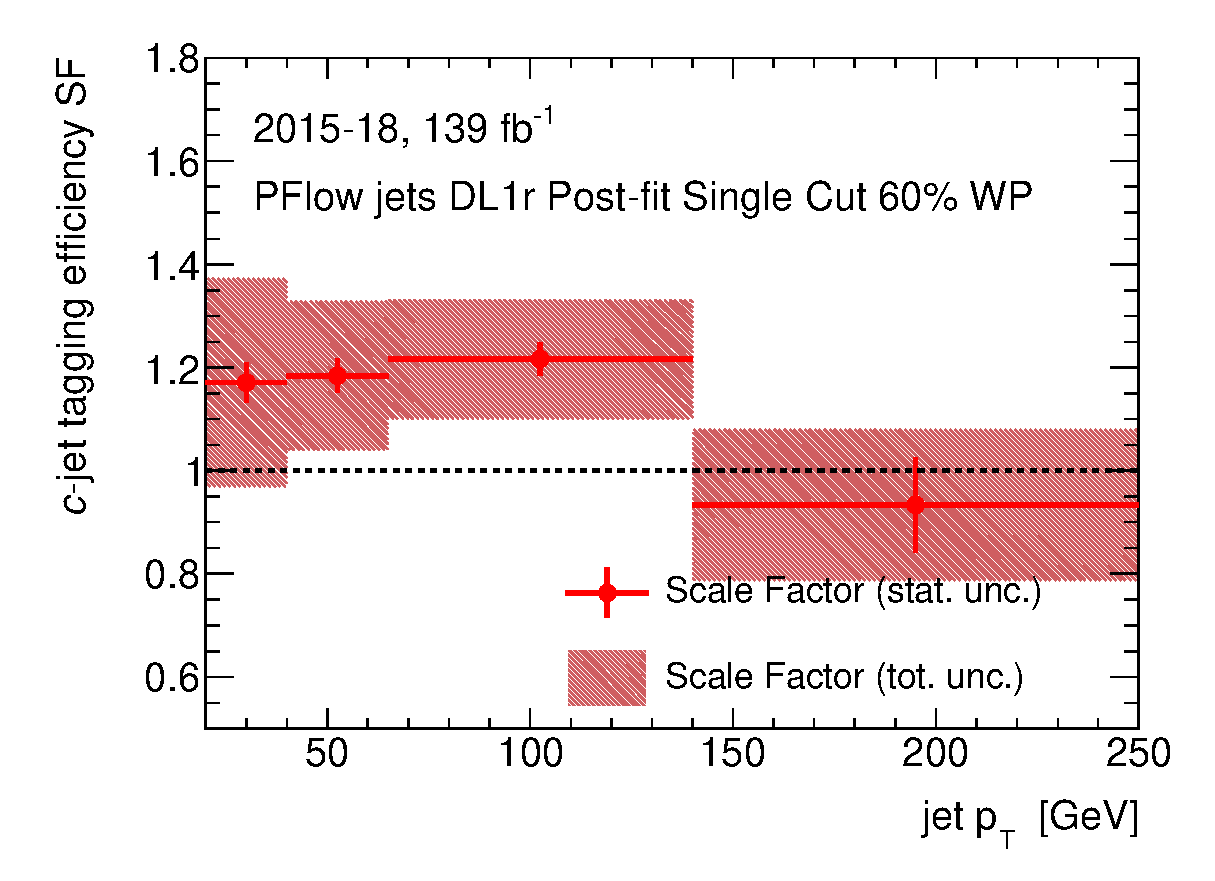
\includegraphics[width=1\textwidth]{FTAG_plots/DL1rallPFlowDec/SF60.eps}
    \caption{60\% working point}
    \end{subfigure}
    \begin{subfigure}[t]{.35\linewidth}
    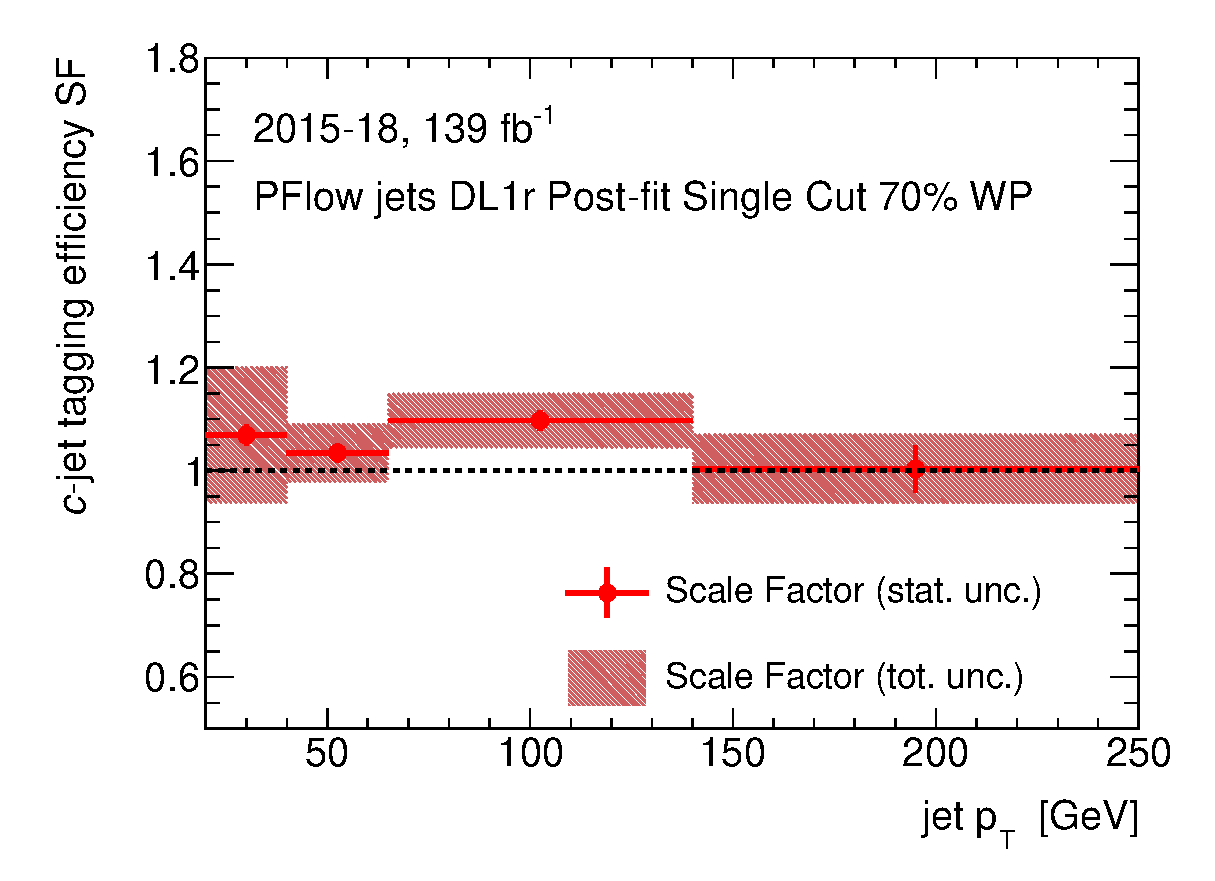
\includegraphics[width=1\textwidth]{FTAG_plots/DL1rallPFlowDec/SF70.eps}
    \caption{70\% working point}
    \end{subfigure}
    \begin{subfigure}[t]{.35\linewidth}
    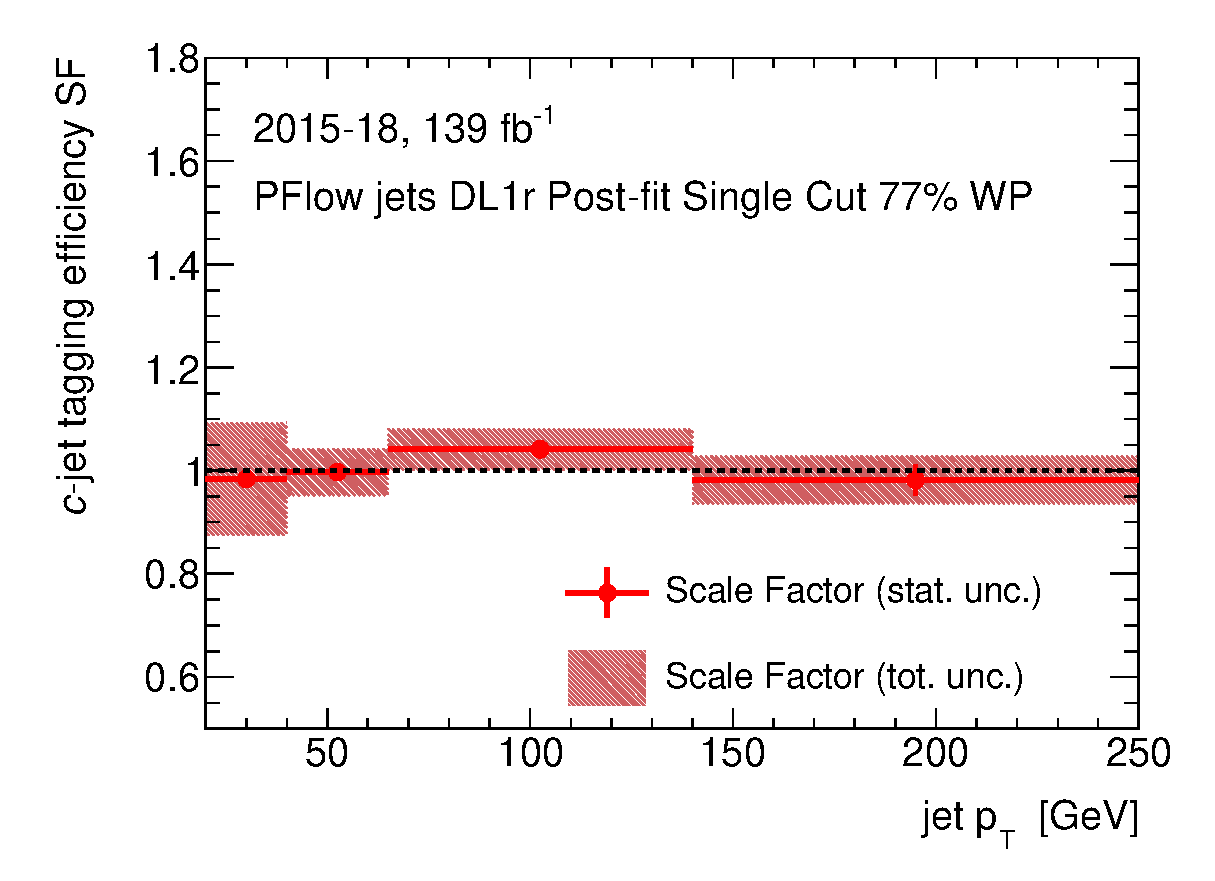
\includegraphics[width=1\textwidth]{FTAG_plots/DL1rallPFlowDec/SF77.eps}
    \caption{77\% working point}
    \end{subfigure}
    \begin{subfigure}[t]{.35\linewidth}
    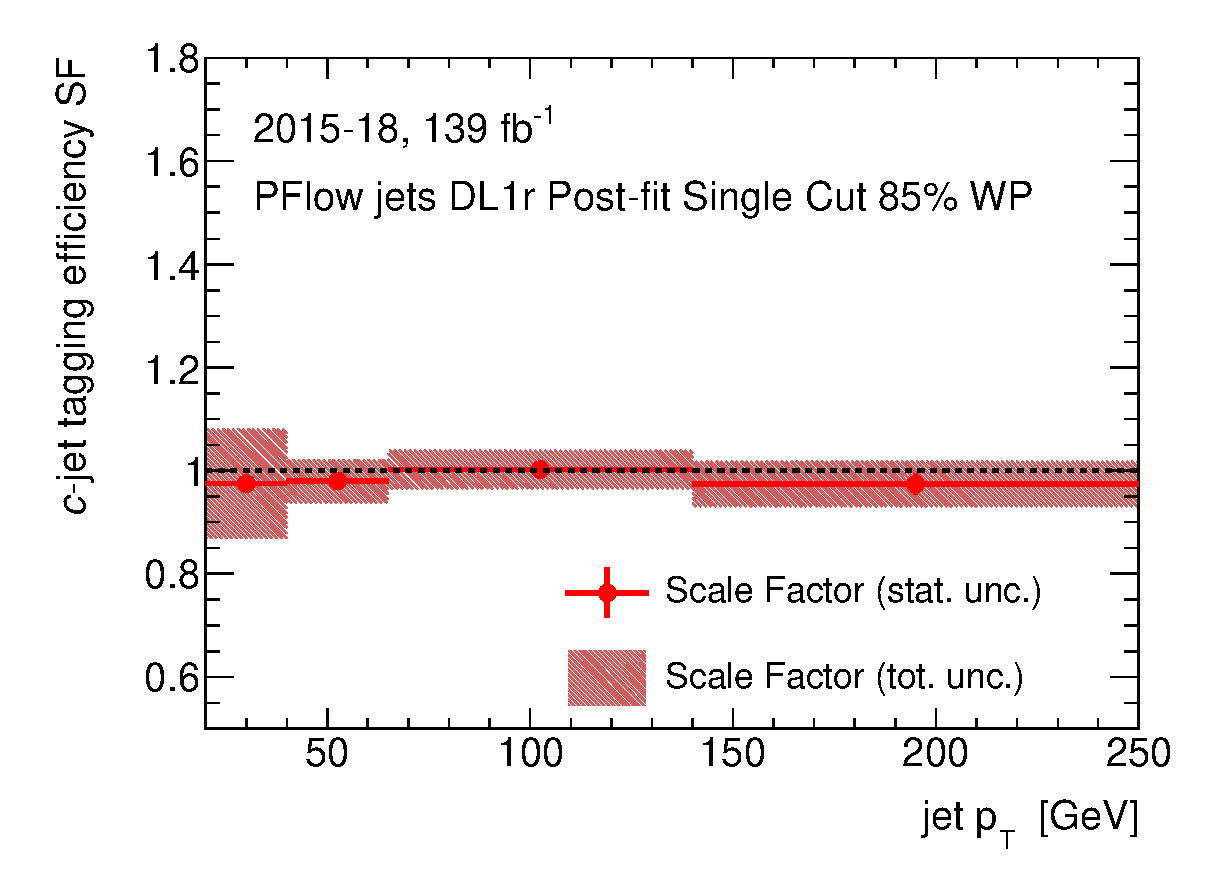
\includegraphics[width=1\textwidth]{FTAG_plots/DL1rallPFlowDec/SF85.eps}
    \caption{85\% working point}
    \end{subfigure}
    \caption{Charm-jet scale factors for the PFlow jets collection with 
    the DL1r tagger.} \label{fig:Dec_SF_PFlow_DL1r}
    \end{figure}	

\Large{3.7\ Title of Representative Academic Achievements}\\
\newline
\normalsize
Combination of searches for non-resonant and resonant Higgs boson pair production in 
the \bbyy, \bbtautau, \bbbb\ decay channels using pp collisions at $\sqrt{s}$ = 13 TeV with the ATLAS detector\\
\newline
\Large{3.8\ Abstract of Representative Academic Achievement}\\
\normalsize
\newline
    I have contributed to a combination of searches conducted for Higgs boson pair production using 
    126--139\ifb of proton-proton collision data recorded with the ATLAS detector at a center-of-mass energy of 
    $\sqrt{s}=\SI{13}{\tev}$ at the LHC. Three searches for pairs of Higgs bosons, 
    in the $b\bar{b}\gamma\gamma$, $b\bar{b}\tau^{+}\tau^{-}$, and $b\bar{b}b\bar{b}$ 
    final states, are included in this combination. 
    The non-resonant interpretation uses 
    results from the $b\bar{b}\gamma\gamma$ and $b\bar{b}\tau^{+}\tau^{-}$ searches, 
    while the resonant interpretation uses results from all three searches. 
    No statistically significant excess above the Standard Model expectation has been found. 
    Upper limits are set on the production rate of non-resonant Higgs boson pairs, at the 95\% confidence level,
    assuming Standard Model kinematics. 
    The combined limit sets the \textbf{most stringent} upper limits on the non-resonant $HH$ 
    production cross-section to date, representing the current \textbf{best sensitivity} in searches for 
    $HH$ production. 
    \newline

\Large{3.9\ Main Content of the Representative Academic Achievements}\\
\normalsize
\newline
    The observed (expected) combined upper limit is found to be 3.1 (3.1) 
    times the Standard Model prediction. The limits set by individual channels and combined 
    are shown in Table~\ref{tab:results_nonres_exp_limits}.
    \begin{table}[htbp]
        \sisetup{}
        \begin{center}
        
        \begin{tabular}{l
        S[round-mode=places, round-precision=1]|
        S[round-mode=places, round-precision=1]
        S[round-mode=places, round-precision=1]
        S[round-mode=places, round-precision=1]
        S[round-mode=places, round-precision=1]
        S[round-mode=places, round-precision=1]
        }
        \toprule
        & {Obs.} & $\SI{-2}{\sigma}$ & $\SI{-1}{\sigma}$ & {Exp.} & $\SI{+1}{\sigma}$ & $\SI{+2}{\sigma}$ \\
        \midrule
        % {cross-section} & & & & & & & \\
        % % \bbbb & $-$ & $4.806748$ & $6.453069$ & $8.955687$ & $12.514435$ & $16.953666$ \\
        % \bbtautau &    4.126402 &           1.871041 &           2.511876 &    3.486028 &           4.973379 &           7.015396 &  2.995979 &  2.312411 & \\
        % \bbyy &    4.058352 &           2.905606 &           3.900781 &    5.413576 &           7.998831 &          11.986507 &  5.327046 &  3.790706 &  \\
        % Combined &    2.786297 &           1.510250 &           2.027514 &    2.813821 &           4.002772 &           5.619012 &  2.486833 &  1.682553 &  \\
        % \midrule
        %{Signal strength} & & & & & & & \\
        \bbyy &         4.308676 &           3.083336 &           4.139384 &    5.744714 &           8.821852 &          14.253823  \\
        \bbtautau &    4.644017 &           2.072931 &           2.782913 &    3.862179 &           5.871155 &           9.380173   \\
        \midrule
        Combined &    3.056996 &           1.657194 &           2.224786 &    3.087599 &           4.657015 &           7.342502   \\
        
        \bottomrule
        \end{tabular}
        \caption{Observed and expected $\SI{95}{\percent}$ C.L.\ upper limits on the 
        signal strength for SM \HH production derived from the \bbtt and \bbyy searches,
        and their statistical combination. 
        }
        \label{tab:results_nonres_exp_limits}
        \end{center}
        
        \end{table}

    Upper limits on the production cross-section of a heavy scalar resonance decaying 
    to two Standard Model Higgs bosons are set at 95\% confidence level between 
    1.1 and 595 fb (1.2 and 392 fb) in observation (expectation), 
    depending on the resonance mass, $m_X$, within the studied mass 
    range $\SI{251}{\gev}\le m_X \le\SI{3}{\tev}$.  
    The limits set on the resonance is shown in Figure~\ref{fig:spin0_obs_limits}

    \begin{figure}[htbp]
        \centering
        \includegraphics[height=0.45\textheight]{DiHiggs/plots/upperlimit_xsec_spin0_json_obs_fullcorr.pdf}
        %\subfloat[Local $p$-value]{\includegraphics[width=0.5\textwidth]{figures/pvalue/\pvaluedate/spin0/spin0_local_pvalue.pdf}}
        \caption{Expected and observed 95\% C.L.\ upper limits on $\sigma(X \rightarrow HH$ 
        for a spin-0 resonance as a function of its mass \mX in the \bbyy, \bbtt and \bbbb searches, 
        and their statistical combination. 
        % The discontinuities in the limit visible in the range
        %  $\mX < \SI{400}{\gev}$ are caused by the partial availability of the different analysis limits on 
        %  a point-by-point basis, which are provided only for the \bbyy search at the weakest limit points. 
        %  Further details can be found in \Tabrange{\ref{tab:spin-0-individual-fullcorr-1}}{\ref{tab:spin-0-individual-fullcorr-4}} in the appendix.
        }
        \label{fig:spin0_obs_limits}
    \end{figure}
    
    The Higgs boson self-coupling, $\lambda_{HHH}$, provides 
    direct access to the shape of the Higgs potential, and its measurement is a \textbf{primary physics goal} of 
    the LHC and its forthcoming upgrade, the High Luminosity LHC.
    Modifications to the Higgs boson self-coupling can 
    occur through BSM, which can lead to an enhancement of the rate of Higgs boson 
    pair-production and modifications of the kinematics of the process. 
    For example, changing the sign of the Higgs boson trilinear self-coupling with respect to the 
    Standard Model expectation would quadruple the \HH production rate. It is estimated 
    that the Higgs boson trilinear self-coupling can be measured to a 
    precision of 50\% at the HL-LHC by combining results from both ATLAS and CMS. 
    
    The value of the Higgs boson trilinear self-coupling modifier 
    $\kappa_{\lambda} \equiv \lambda_{HHH}/\lambda_{\mathrm{SM}}$ is excluded outside the observed (expected) range 
    $-1.0 \le \kappa_{\lambda} \le 6.6$ ($-1.2 \le \kappa_{\lambda} \le 7.2$) 
    at 95\% confidence level. The limit result is shown in Figure~\ref{fig:kl_scan_combined}.
    \newline
    \begin{figure}[htbp]
        \centering
        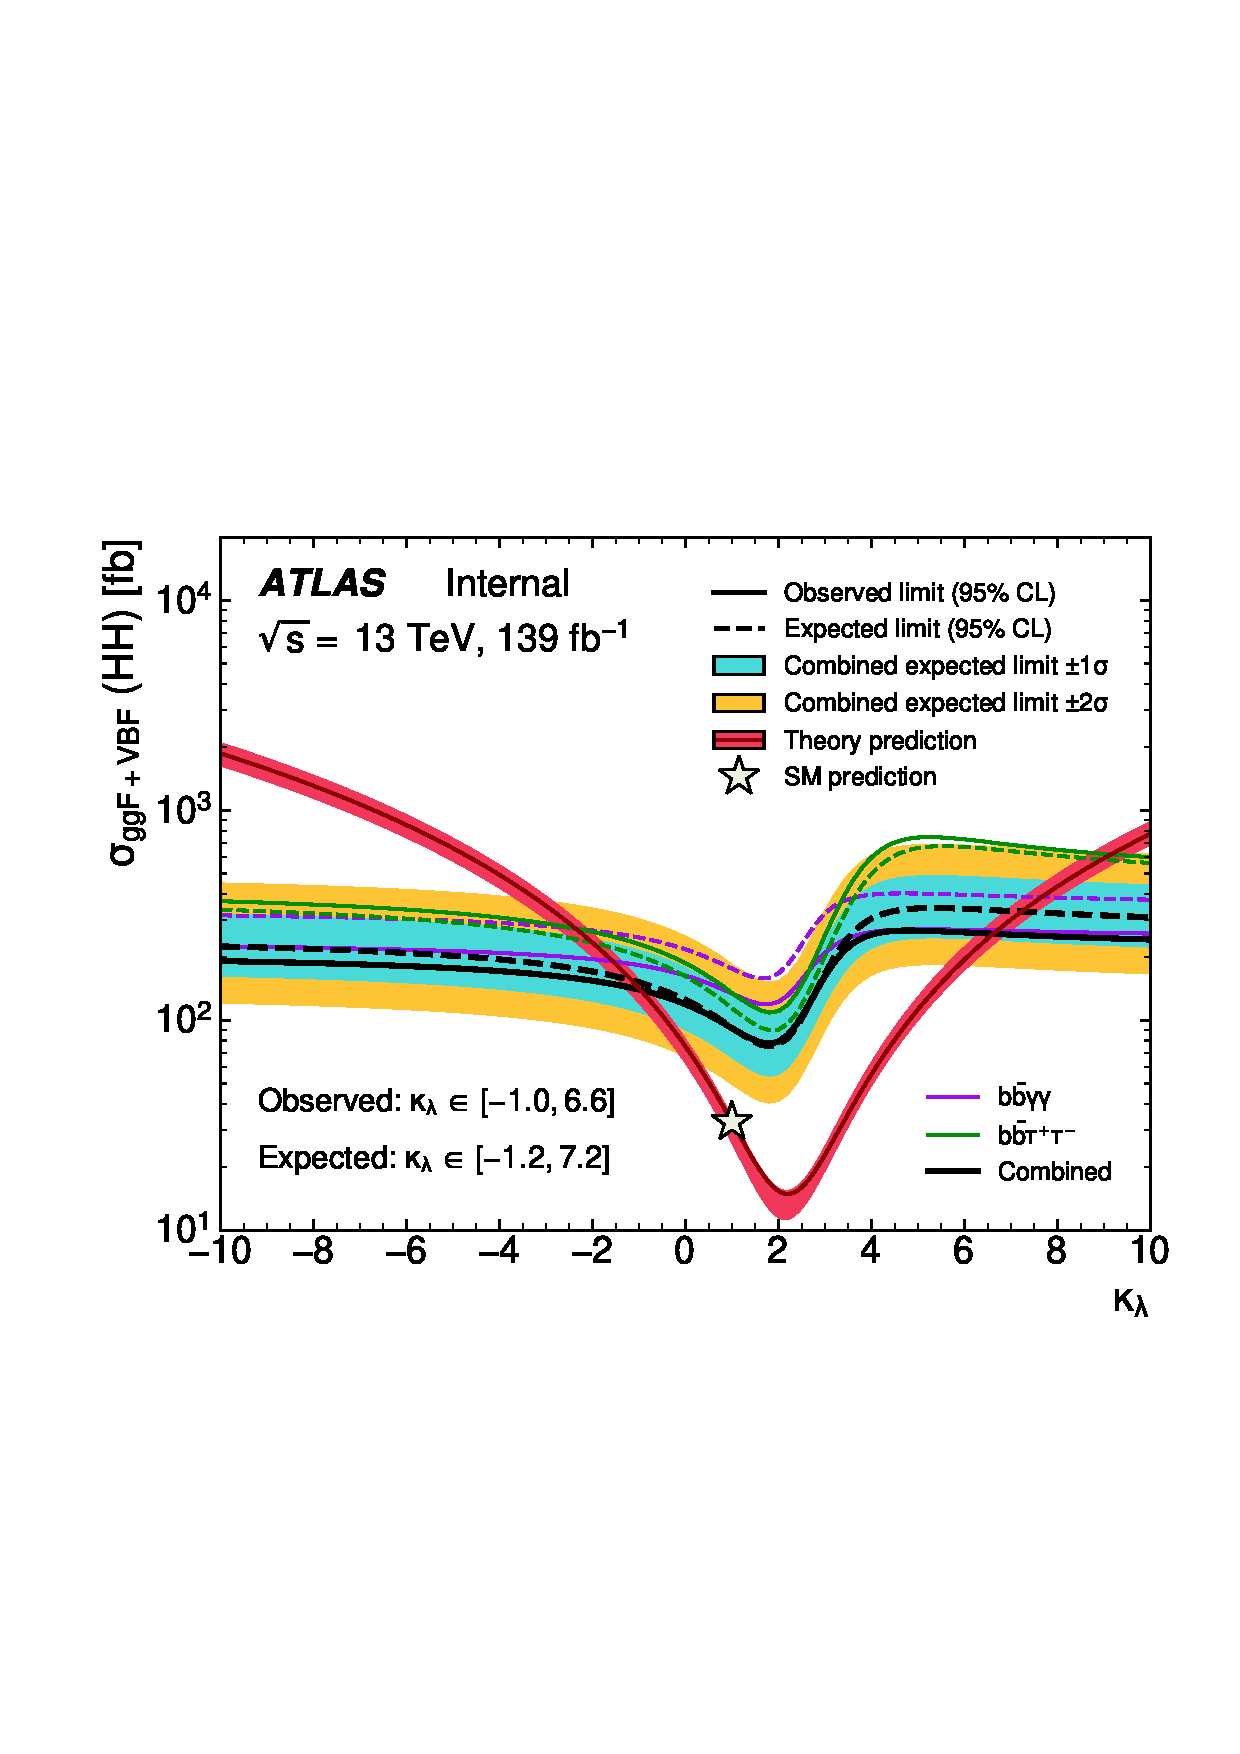
\includegraphics[width=0.8\textwidth]{DiHiggs/plots/kl_scan/20210926/all_channels_kl_scan_mH125.pdf}
        \caption{Observed and expected 95\% CL exclusion limits on non-resonant $\sigma(pp \rightarrow HH)$ 
        as a function of $\kappa_\lambda$ for the individual channels and the combination of \bbtt and \bbyy.
        }
        \label{fig:kl_scan_combined}
    \end{figure}   

\Large{3.10\ Title of Representative Academic Achievements}\\
\normalsize
\newline
HEFT interpretation of Higgs boson pair searches in \bbyy, \bbtt\ final states and their combination in
ATLAS\\
\newline
\Large{3.11\ Abstract of Representative Academic Achievement}\\
\normalsize    
\newline
    I have worked on setting limits on Higgs Effective Field Theory (HEFT) benchmark models 
    and couplings based on the searches for $HH$ production in the \bbyy and \bbtautau final states, 
    and their combination. The searches make use of $139$ $\textrm{fb}^{-1}$ of proton-proton collision 
    data recorded with the ATLAS detector at a centre-of-mass energy of $\sqrt{s}=13$ TeV at the LHC. 
    Upper limits on the $HH$ production cross-section are set on seven HEFT benchmark models at the $95$\% confidence level, 
    with observed (expected) limits ranging from $50.2$ ($45.5$) fb to $133.6$ ($133.5$) fb. 
    Exclusion limits are also set on two BSM coupling parameters, 
    $c_{gghh}$ and $c_{tthh}$, described in HEFT, excluding values outside the observed (expected) 
    ranges of [$-0.3, 0.4$] ([$-0.3, 0.3$]) and [$-0.2, 0.6$] ([$-0.2, 0.6$]), respectively, at the 95\% confidence level.
    This is the \textbf{first ever} dedicated search for these two BSM couplings, and represents the \textbf{leading edge} of 
    exploration for new physics.
\newline

\Large{3.12\ Main Content of the Representative Academic Achievements}\\
\normalsize
\newline
Effective Field Theories (EFT) provide a model-independent approach to parametrise the effects of 
candidate BSM theories that reduce to the SM at low energies. This study focuses on the HEFT framework, where the 
Lagrangian is organised following the guidance of chiral perturbation theory and 
where the low-energy dynamics of electroweak symmetry breaking are described using a nonlinear 
realization of $SU(2)\times U(1)$. In this formalism, anomalous Higgs boson couplings are 
expected to be the dominant effects on new physics in the electroweak sector.
Deviations from SM predictions can potentially be observed via $HH$ production using the HEFT framework.

In the HEFT Lagrangian, ggF $HH$ production is described at LO with 
5 operators and their corresponding Wilson coefficients: $c_{hhh}, c_{tth}, c_{tthh}, c_{ggh}$ 
and $c_{gghh}$. The $c_{hhh} = \lambda_{HHH} / \lambda^{\text{SM}}_{HHH}$ and 
$c_{tth} = \lambda_{ttH} / \lambda^{\text{SM}}_{ttH}$ coefficients 
represent the coupling modifiers for the Higgs boson self-coupling and top-quark 
Yukawa coupling ($\lambda_{ttH}$). The remaining Wilson coefficients affect respectively 
the $ttHH$, $gHH$ and $ggHH$ vertex interactions and introduce three non-SM LO Feynman 
diagrams for ggF $HH$ production shown in Figure~\ref{fig:HEFT_diagrams_o6}.
The HEFT Lagrangian reduces to the SM Lagrangian for $c_{hhh} = c_{tth} = 1$ 
and $c_{tthh} = c_{ggh} = c_{gghh} = 0$, when the Higgs boson self-coupling 
and top-quark Yukawa coupling have SM values and none of the BSM production modes are present. 
% therefore the HEFT Lagrangian reduces to the SM Lagrangian.
% when $c_{hhh} =c_{tth} = 1$ and $c_{tthh} = c_{ggh} = c_{gghh} = 0$.
%The three non-SM LO Feynman diagrams for $HH$ production through gluon-gluon fusion, introduced in HEFT, are described by the Feynman diagrams shown in \Fig{\ref{fig:HEFT_diagrams_o6}}.
%The HEFT formalism allows us to make a more general measurement of the Higgs self-coupling and explore different BSM scenarios by simultaneously varying multiple Wilson coefficients \cite{Cohen:2020xca}.
Higgs boson pair production is the \textbf{most promising process} to measure the 
Higgs boson self-coupling because it gives access to $c_{hhh}$ at tree level.
Furthermore the \HH process gives \textbf{unique access} to 
the two other Wilson coefficients, $c_{tthh}$ and $c_{gghh}$.
% On the contrary, single Higgs boson processes have better sensitivity to the remaining two coefficients, $c_{tth}$ and $c_{ggh}$.
The HEFT formalism allows us to interpret general searches in different BSM scenarios 
by simultaneously varying multiple Wilson coefficients. 
%\usepackage[utf8]{inputenc}
%\usepackage{tikz}
%\usepackage[compat=1.1.0]{tikz-feynman}
%\usepackage{subcaption}
%\usepackage{geometry}

\definecolor{hh_pink}{HTML}{F2385A}
\definecolor{hh_blue}{HTML}{343844}
\definecolor{hh_med_turq}{HTML}{36B1BF}
\definecolor{hh_lgt_turq}{HTML}{4AD9D9}
\definecolor{hh_whte}{HTML}{E9F1DF}
\definecolor{hh_yllw}{HTML}{FDC536}
%\definecolor{hh_gren}{HTML}{125125}
\definecolor{hh_gren}{HTML}{00CC00}


%\usepackage[EULERGREEK]{sansmath}
%\usepackage{floatrow}
%\DeclareFloatFont{henry}{\sffamily\sansmath}
%\floatsetup[figure]{font=henry}

\begin{figure}[tbh!]
    \centering                          
    \begin{subfigure}[t]{0.3\textwidth}
        \centering
        \begin{tikzpicture}
               \begin{feynman}
                
                \vertex(g1) at (-2.3, -1.3) {\(\mathbf{g}\)};
                \vertex(g2) at (-2.3, 1.3) {\(\mathbf{g}\)};
                \vertex (ggh) at (-0.8, 0);
                \vertex (h1) at (0.8, 0);
                \vertex (h2) at (2.2, 1.3) {\(\mathbf{H}\)};
                \vertex (h3) at (2.2, -1.3) {\(\textbf{H}\)};

                \diagram*{
                    (g1) -- [gluon, thick] (ggh),
                    (g2) -- [gluon, thick] (ggh),
                    (ggh) -- [scalar, thick, edge label'=\(\textbf{H}\)] (h1) -- [scalar, thick] {(h2), (h3)}
                };
                
            \end{feynman}

        \filldraw [hh_blue] (-0.8, 0) circle (3pt);
        \node[hh_blue, scale=1.25] at (-0.8, 0.6) {\(c_{ggh}\)};
        \filldraw [hh_pink] (0.8, 0) circle (3pt);
        \node[hh_pink, scale=1.25] at (0.8, 0.6) {\(c_{hhh}\)};
        
        \end{tikzpicture}
    \caption{ggh and hhh}
    \end{subfigure}
    \begin{subfigure}[t]{0.3\textwidth}
        \centering
        \begin{tikzpicture}
            \begin{feynman}

		\vertex(g1) at (-1.6, -1.3) {\(\mathbf{g}\)};
                \vertex(g2) at (-1.6, 1.3) {\(\mathbf{g}\)};
                \vertex (t) at (0.0, 0);
		\vertex (h1) at (1.6, 1.3) {\(\mathbf{H}\)};
                \vertex (h2) at (1.6, -1.3) {\(\textbf{H}\)};

                \diagram*{
                    (g1) -- [gluon, thick] (t),
                    (g2) -- [gluon, thick] (t),
                    (t) -- [scalar, thick] {(h1), (h2)}

		};

            \end{feynman}

        \filldraw [hh_gren] (0.0, 0.0) circle (3pt);
        \node[hh_gren, scale=1.25] at (0.0, 0.6) {\(c_{gghh}\)};

        \end{tikzpicture}
    \caption{gghh}
    \end{subfigure}
    \begin{subfigure}[t]{0.3\textwidth}
        \centering
        \begin{tikzpicture}
            \begin{feynman}

                \vertex(g1) at (-2.5, -1.25) {\(\mathbf{g}\)};
                \vertex(g2) at (-2.5, 1.25) {\(\mathbf{g}\)};

                \vertex (t1) at (-1.0, -1.25);
                \vertex (t2) at (-1.0, 1.25);
                \vertex (t3) at (0.5, 0);

                \vertex (h1) at (2.0, 1.25) {\(\mathbf{H}\)};
                \vertex (h2) at (2.0, -1.25) {\(\textbf{H}\)};

                \diagram*{
                    (g1) -- [gluon, thick] (t1),
                    (g2) -- [gluon, thick] (t2),

                    (t1) -- [fermion, thick] (t2) -- [fermion, thick] (t3) -- [fermion, thick] (t1),

                    (t3) -- [scalar, thick] {(h1), (h2)}

                };

            \end{feynman}

        \filldraw [hh_yllw] (0.55, 0) circle (3pt);
        \node[hh_yllw, scale=1.25] at (0.55, 0.6) {\(c_{tthh}\)};

        \end{tikzpicture}
    \caption{tthh}
    \end{subfigure} \\                                                                                                                                                                                     

    \caption[Feynman diagrams, gluon-gluon fusion di-Higgs production]{BSM HEFT leading order Feynman diagrams for Higgs boson pair production through gluon-gluon fusion.}% In SM, $c_{tth}=c_{hhh}=1$ and $c_{tthh}=c_{ghh}=c_{gghh}=0$.}
    \label{fig:HEFT_diagrams_o6}
\end{figure}


The 95\% CL upper limits on the ggF \HH cross-section for the combination 
of the \hhtobbyy and \hhtobbtt searches for the HEFT shape benchmarks are shown 
on \Fig{\ref{fig:results:combined_BM}}.
The most stringent limits are set for benchmark~7 with an observed (expected) 
limit of 50.2~fb (45.5~fb) while the least are for benchmark~2 
with an observed (expected) limit of \SI{133.6}{fb} (\SI{133.5}{fb}).
The expected limits assume no \HH production.
The 95\% CL combined upper limits on the ggF \HH cross-section as a 
function of \cgghh and \ctthh are shown in \Fig{\ref{fig:combined_scans}}. 
The observed (expected) 95\% CL intervals on $\cgghh$ and $\ctthh$ are 
$-0.3 < \cgghh  < 0.4$ ( $-0.3 < \cgghh  < 0.3$) and $-0.2 < \ctthh < 0.6$ ( $-0.2 < \ctthh < 0.6$).
\newline

\begin{figure}[tbh!]
    \centering
    \includegraphics[width=0.6\textwidth]{casual plots/combined_benchmark_limit.pdf}
    \caption{Observed and expected 95\% CL upper limit on $\sigma_{ggF}$ for the seven HEFT shape benchmarks and SM  obtained from \bbtautau and \bbyy analyses, and their combination. The expected limits assume no \HH production.}
    \label{fig:results:combined_BM}
\end{figure}

\begin{figure}[tbh!]
    \centering
    \begin{subfigure}[t]{0.48\textwidth}
        \centering
        \includegraphics[width=\textwidth]{casual plots/combined_cgghh_limit_scan.pdf}
        \caption{}
    \end{subfigure}
    \begin{subfigure}[t]{0.48\textwidth}
        \centering
        \includegraphics[width=\textwidth]{casual plots/combined_ctthh_limit_scan.pdf}
        \caption{}
    \end{subfigure}
    \caption{95\% CL upper limits on the ggF \HH cross-section as a function of the \cgghh (a) and \ctthh (b) HEFT Wilson coefficients obtained for the \hhtobbyy and \hhtobbtt combination.
    The expected limits assume no \HH production.
    The theory prediction curve in red presents the situation where all Wilson coefficients are set to their SM values except for the one under study.
    }
    \label{fig:combined_scans}
\end{figure}


\Large{\textbf{4.Postdoctoral Research Project }}\\
\newline
\Large{4.1\ Title of Postdoctoral Research Project}\\
\newline
\normalsize
Searching for double Higgs with the CMS detector \\
\newline
\Large{4.2\ Abstract of Postdoctoral Research Project}\\
\newline
\normalsize
In my postdoctoral research, 
I will play a prominent role in the areas of physics related to the Higgs boson 
(Higgs decays to muon pairs, double Higgs production, precision measurements of Higgs properties) and 
Dark Matter using machine learning techniques.
I will also participate the efforts of the MTD detector or/and the GEM detector as a part of the CMS Phase II upgrade.\\
\newline
\Large{4.3\ Content of Postdoctoral Research Project(max. 10 pages in total, including time plan, all tables/figures and references, etc.)}\\
\newline
\normalsize
Currently, there is no public result available using the full Run2 CMS data to search for di-Higgs production
in the \bbtt\ channel, nor combination of results with sensitivity close to ATLAS result. 
Searches for di-Higgs production using \bbtt\ final states have great potential and once combined with the ALTAS results, 
the constrain on the di-Higgs production cross-section will approximately be around two times the SM expectation, 
and if we are lucky enough, the observed limit could go even lower, approaching the SM expectation. This will be a very strong 
constrain on new phsics and will guide us in future analysis. 
In particular, the sensitivity of ATLAS di-Higgs searches in \bbtt\ channel is limited by large background systematics.  
During the research project, I will take the leading role in di-Higgs searches using CMS data in various final
states, not limited to the \bbtt\ channel. I will be improving the analysis by minimising the systematic errors,
and developing better techniques for background estimation, such as using data-driven or more advanced machine learning
techniques.
I will also utilise my expertise in multivariate techniques in other areas
of Higgs boson research, such as measurement of Higgs boson decaying to muon pairs, and precision measurements
of Higgs properties. If time allows, I will also join the effort in searches for dark matter. 


In the HL-LHC, the integrated luminosity will increases by a factor of 5 leading to much quicker data taking 
but also severe pileup that challenges the measurement precision.
To deal with this dense environment, CMS planned and is building a new timing detector.
% MTD expecting to improve the timing resolution by 3 orders of magnitude.
This device will bring a completely new capability to CMS — the ability to measure precisely the production 
time of minimum ionizing particles (MIP) for use in disentangling the approximately 200
nearly-simultaneous ``pileup'' interactions that will occur in each bunch crossing of the LHC. It
also provides new capabilities for charged hadron identification and the search for long-lived
particles.
In 2021, CMS China officially joined MTD efforts where Peking University has joined MTD barrel project.
I will join the CMS Peking U.\ group and contribute to development of technicalities of sensors and procurement, and 
the assemble of sensor modules, detector modules and trays as well as the installation of MTD barrel
in the tracker chamber at CERN.

Gas electron multiplier (GEM) detectors represent a new muon system in CMS, 
in order to complement the existing systems in the endcaps. 
The forward region is the part of CMS most affected by large radiation doses and high event rates, 
and we foresee these parameters to be again enhanced during phase II of the LHC. 
The GEM chambers will provide additional redundancy and measurement points, 
allowing a better muon track identification and also wider coverage in the very forward region.
The production of detector modules are distributed of production among several sites outside CERN, 
one of which will be at CMS Peking group. 
I will join the effort of the production of the detector modules, supervised by Doc.\ Qiang Li,
contribute to the R\&D projects, including DAQ, cosmic-ray tests, beam tests, assembling, software, etc.






\end{document}